\begin{listequbox}
  {f(x) = \dfrac{e^x-e^{-x}}{e^x+e^{-x}}}{equtanh}{Tanh function}
\end{listequbox}

\begin{grafica}[H]
\center
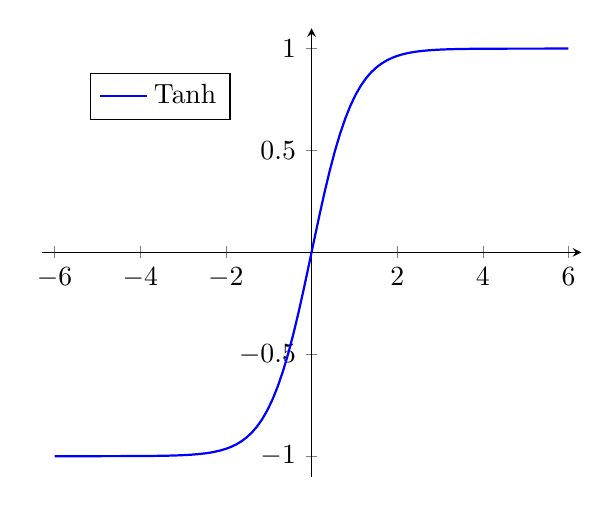
\begin{tikzpicture}
  \begin{axis}[
    xmin=-6.3,xmax=6.3,
    ymin=-1.1,ymax=1.1,
    legend style={at={(0.35,0.9)}},
    axis lines=center
    ]
    \addplot[color=blue,samples=100,domain=-6:6,thick]{(exp(x)-exp(-x))/(exp(x)+exp(-x))};
    \addlegendentry{Tanh}
  ]
  \end{axis}
\end{tikzpicture}
\caption{Tanh function}
\end{grafica}

\textbf{Charasterisics:}

\begin{itemize}
  \item Domain: $(-\infty,\infty)$
  \item Range: $(-1,1)$
\end{itemize}
